\subsection{Matching}
\label{subsec_method_matching}

The following sections show the approach for matching (i.e. finding the same entity in different datasets) and merging (i.e. integrating two different datasets about the same entity into one.)

\subsubsection{Problem statement}
After loading the initial dataset into the database, the task is to integrate other datasets to create a whole dataset with more information than a single one can provide on their own.
% TODO: Why IMDB?
However, simply dumping the second dataset into the database would lead to duplicated entries and thereby decreasing the overall quality of the database.
Thus, the datasets need to be aggregated and unified by looking for a match for each new entry in the old dataset.
Potentially, this has to be done for matching every entry, such as movies, actors, characters and more but the next parts focus on matching just movies to each other.

A first approach is to match movies only by their name.
However, only using the name as a matching criteria yields multiple problems, such as:
\begin{itemize}
	\item different movies having the same name e.g.
	\begin{itemize} 
        \item The Avengers (2012) vs. The Avengers (1998)
        \item Casino Royale (1967) vs. Casino Royale (2006)
    \end{itemize}
	\item same movies having different names in different datasets e.g.
	\begin{itemize} 
        \item Spelling errors: Batman vs Badman
        \item Localization: The Internship vs. Prakti.com
        \item Formatting: The Italian Job vs. Italian Job, The
     \end{itemize}
\end{itemize}
Hence, a more sophisticated approach needs to be developed to increase the quality of the dataset.

\subsubsection{Matching using actor overlap}
In general, the matching algorithm must satisfy two requirements:
\begin{enumerate}
	\item{High precision:} A movies should not be matched to a wrong movie, as this decreases the quality of the dataset. We want to find many matches, but it is important not to add too many wrong matches.
	\item{Performance:} With thousand of movies in each new dataset, matching should not take too long, as there are thousands of movies to match (e.g. TMDB has ca. 170,000 (TODO Check this number) movies to match.
	If each movie takes just 1 minute to match, the whole process for TMDB already takes $171,000~movies * 1 \frac{minute}{movie} * \frac{1}{1440} \frac{days}{minute} \approx 119~days$.
	This is just one data source, and only the current set of movies (remember, there are new movies every day from all data sources, which need to be merged)).
\end{enumerate}

This leads to two consequences: First, a certain level of confidence needs to be reached to match two movies to each other. Otherwise, it is impossible to detect movies, which are not matchable, because they are not in the database.
Second, comparing each movie with all movies in the database is not feasible.

This paper proposes the idea to first find a small list of movies that could be a match (henceforth called candidates) and then calculate a score for each of these candidates, which is based on the actors . Details are described in the following paragraphs.

Figure \ref{fig_matching_general} shows the general matching procedure:
First, we pass through each new movie, that we want to match.
For each movie $n_i \in N$ ($N$ is the set of movies we still need to match), we first select a small set of movies $C_{i}$ that could be a match (henceforth called candidates).
Then we calculate a score, which captures the similarity between $n_i$ and each $m_j \in C_i$.
This score is mostly based on the actor information we have about the two movies.
Finally, we choose the movie with the highest score, if the score is above a certain threshold.

\begin{figure}[ht]
  \begin{center}
  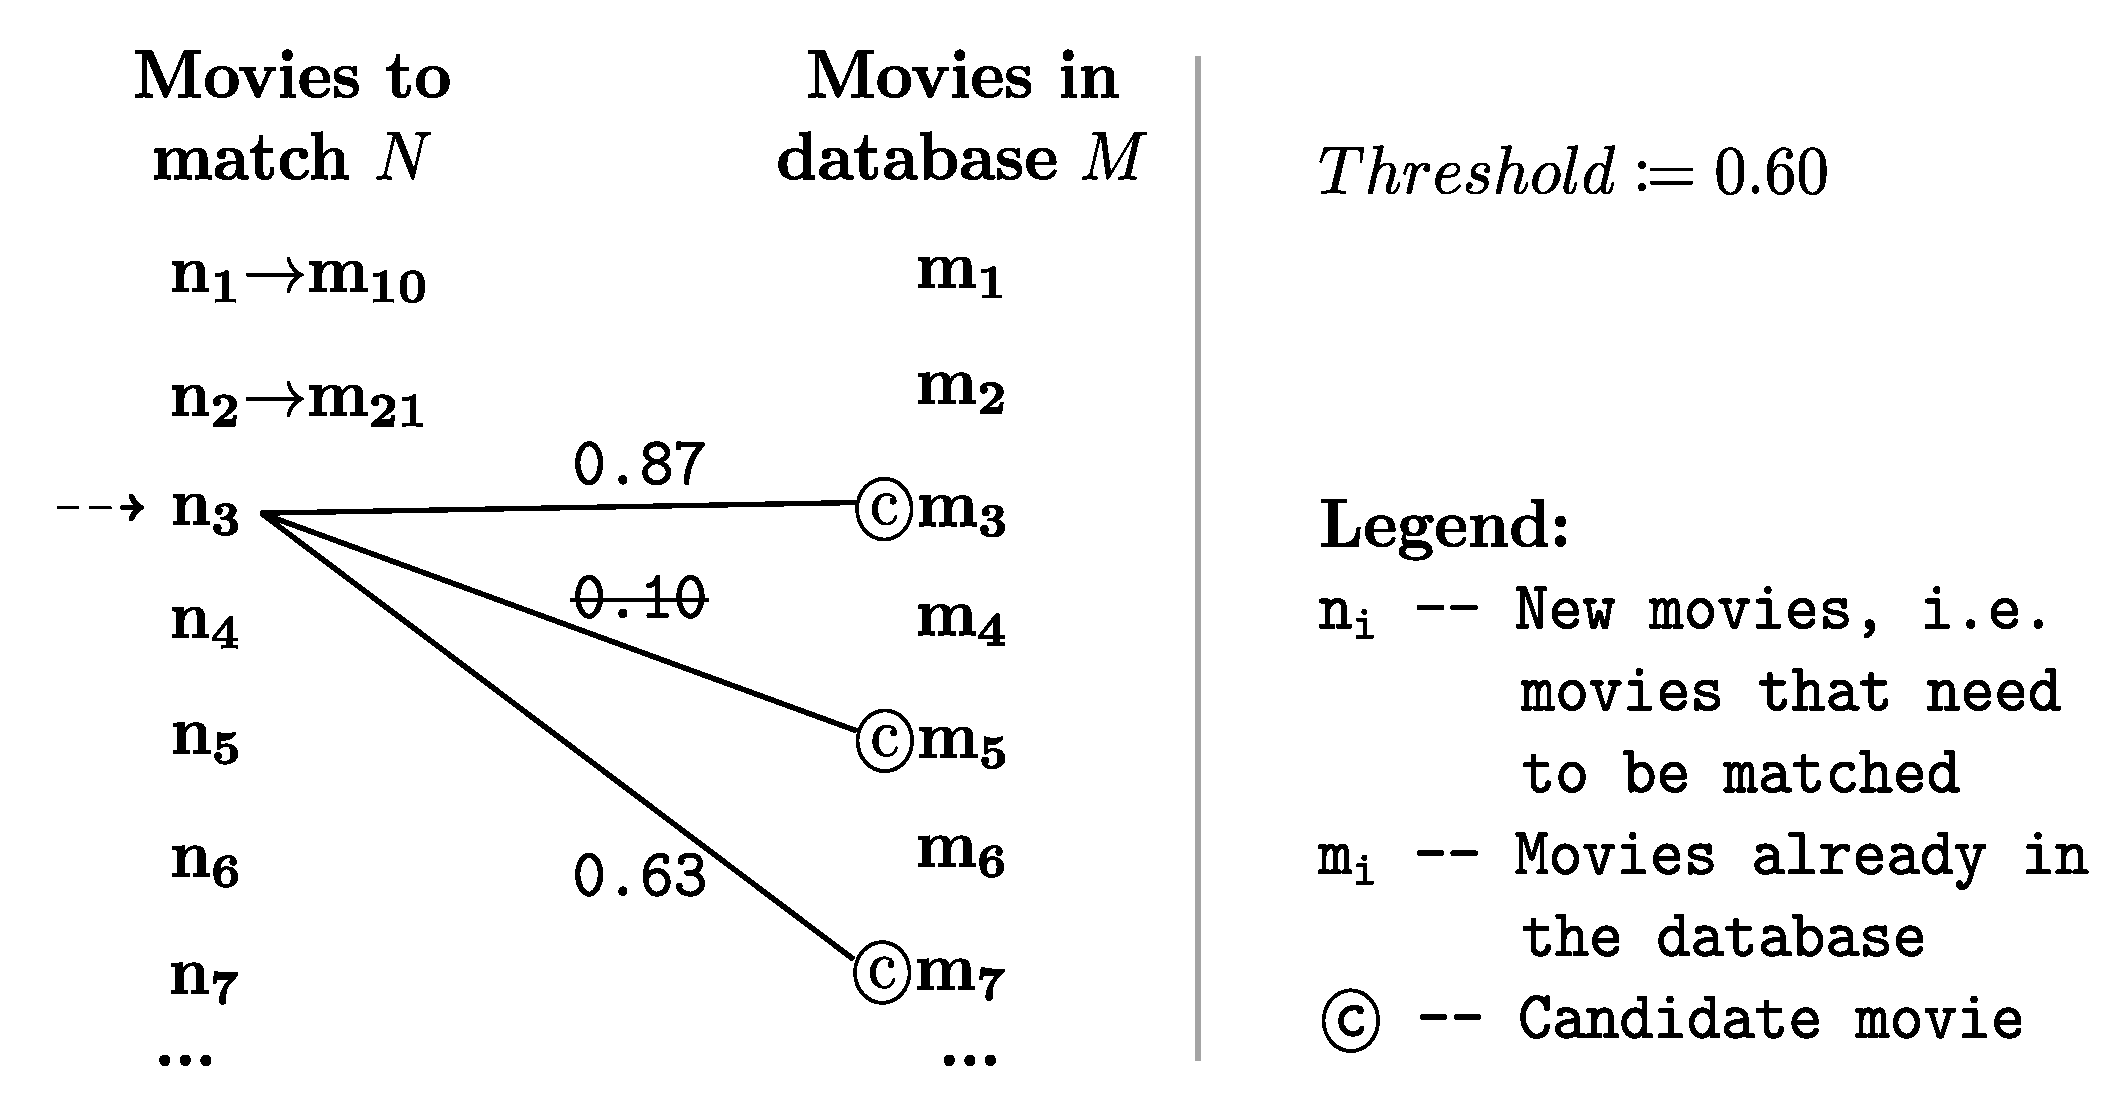
\includegraphics[width=0.8\textwidth]{images/matching_general.pdf}
  \end{center}
  \caption{This shows the general matching procedure. In this case, we would choose movie $m_3$ as a match for $n_3$, because it has the highest score and is above the threshold.}
  \label{fig_matching_general}
\end{figure}

The next paragraphs describe candidate selection and score calculation in detail.

\paragraph{Candidate selection}

The general goal of candidate selection is to reduce the set of all movies in the database to a smaller set of candidates.
There are two constraints working against each other:
\begin{itemize}
	\item The candidate should be as small as possible. This leads to fewer comparisions and thereby increased performance.
	\item The correct movie, i.e. the movie that needs to be matched to our current movie, must be in the candidate set, if it exists in the database.
\end{itemize}
The former would be optimized by returning nothing, the latter by returning everything, so a viable tradeoff has to be found.

The algorithm presented in this paper uses a candidate selection by calculating a pre-score based on the year and the name of a movie.
This two properties have shown to be available in all datasets for all movies.
The pre-score is calculated based on the Levenshtein distance \footnote{The Levenshtein distance between two strings is defined as the amount of edit operations (insertions, deletions, substitutions), which are needed to transform the first string into the second one.} $n_i$ and each $m_j$ and the distance between the years $year(n_i)$ and $year(m_j)$.
Calculating these numbers for all movies in the database can be done efficient enough to provide a fast candidate selection.
These numbers are combined into a score, where the Levenshtein distance is weighted more.
Finally, the best 100 movies are selected as candidates, according to the score computed in the previous step.

Please not, that candidate selection is not matching over the name, because no decisions need to be made between two similar named movies.
Similar named movies are still good candidates, but the matching itself is using a different approach (see following chapter).

TODO: Reword

\paragraph{Score calculation}
After the candidates have been selected, the next step is to find the best match.
For that, the algorithm uses the actor information we have about $n_i$ and each $m_j$ in $C_i$.
Given
\begin{description}
	\item[$n_i$] the movie we want to match,
	\item[$C_i$] the set of candidates for the movie,
	\item[$A_{movie}$] a function, which returns the actor names from a movie in one of our datasets,
	\item[$Levenshtein(s_1, s_2)$] a function, which returns the edit distance (insert, remove, replace) between two strings.
\end{description}
the best match $n_i$ is determined as follows:

\begin{align}
	match(n_i) &=
		\begin{cases}
			best\_match(n_i),~if~score > MIN\_SCORE) \\
			\bot
		\end{cases}\label{aoeq:1}\\
	best\_match(n_i) &=
		\argmax_{m_j \in C_i} score(n_i, m_j)\label{aoeq:2}\\
	score(n_i, m_j) &=
		\frac
			{\left\lvert overlap\_set(A_{n_i}, A_{m_j}) \right\rvert}
			{\left\lvert A_{n_i}) \right\rvert}\label{aoeq:3}\\
	overlap\_set(A_{n_i}, A_{m_j} &=
		\Set*{a_n \in A_n}{\exists a_m \in A_m: Levenshtein(a_n, a_m) < ACT\_DIST}.\label{aoeq:4}
\end{align}

The basic idea, which is shown in equation \ref{aoeq:1}, is to only assume a match, if the score of the best matching movie is above a certain threshold $MIN\_SCORE$.
So $MIN\_SCORE$ determines, when a best matching movie is returned as an actual match.
If its score is too low, the assumption is that the movie is not the right one (i.e. the correct one does not exist in the database).
Thus, nothing is returned.

The best matching movie is defined as the movie from the candidate set, which has the highest score (see equation \ref{aoeq:2}.

The the algorithm's main idea is illustrated in equation \ref{aoeq:3}: Given the movie to match and a candidate, the score's is determined as the fraction of the movie's actor, which can also be found in the candidate movie's actors.

The check whether one actor from one movie is also in the other movie, we do not use strict matching, but rather a fuzzy approach, see \ref{aoeq:4}.
Two actors are considered equal (but only for the sake of matching movies), when their Levenshtein distance is below a certain threshold $ACT\_DIST$.

The main idea of the algorithm is to use the actor overlap between two movies as the main matching criteria.
The Levenshtein distance in \ref{aoeq:4} may not be able to match all actors correctly (i.e. "`Emma Watson"' and "`Emily Watson"' with a distance of three), because similar name problems can occur as with the movie (misspellings, different spelling in different languages, actual similar names for different actors etc.).
However, the idea is that less actors can be matched for different movies and more actors can be matched for the same movie in different datasources.
An evaluation of this approach can be found in section \ref{subsec_evaluation_matching}.

\paragraph{Implementation}
The actual implementation does not only use the actor overlap, but also the overlap for producers, writers and directors.
However, as these sets are usually smaller then the actor set, these overlaps are used with smaller weight than the actor overlap.
Furthermore, the movie name and the year a movie was published is used as the deciding factor between movies, when their actor overlap is equal.

This improvements have shown to produce slightly better results (also see section \ref{subsec_evaluation_matching}).
